\documentclass[12pt,a4paper]{report}

% Kodowanie i język
\usepackage[utf8]{inputenc}
\usepackage[T1]{fontenc}
\usepackage[polish]{babel}
\usepackage{lmodern}

% Marginesy
\usepackage[margin=2.5cm]{geometry}

% Grafika i kolory
\usepackage{graphicx}
\usepackage{xcolor}

% Tabele
\usepackage{booktabs}
\usepackage{longtable}
\usepackage{tabularx}
\usepackage{array}
\usepackage{multirow}

% Listy
\usepackage{enumitem}

% Kod źródłowy
\usepackage{listings}
\usepackage{lstautogobble}

% Hiperłącza
\usepackage[hidelinks,colorlinks=false]{hyperref}

% Nagłówki i stopki
\usepackage{fancyhdr}

% Interlinea
\usepackage{setspace}
\onehalfspacing

% Wcięcia
\usepackage{parskip}
\setlength{\parskip}{0.5em}

% Definicja koloru dla kodu
\definecolor{codeblue}{RGB}{0,102,204}
\definecolor{codegray}{RGB}{128,128,128}
\definecolor{codegreen}{RGB}{0,128,0}
\definecolor{codebg}{RGB}{248,248,248}
\definecolor{codeborder}{RGB}{220,220,220}

% Styl dla kodu
\lstdefinestyle{mystyle}{
    backgroundcolor=\color{codebg},
    commentstyle=\color{codegreen},
    keywordstyle=\color{codeblue}\bfseries,
    numberstyle=\tiny\color{codegray},
    stringstyle=\color{codegreen!60!black},
    basicstyle=\ttfamily\small,
    breakatwhitespace=false,
    breaklines=true,
    captionpos=b,
    keepspaces=true,
    numbers=left,
    numbersep=8pt,
    showspaces=false,
    showstringspaces=false,
    showtabs=false,
    tabsize=2,
    frame=single,
    rulecolor=\color{codeborder},
    autogobble=true
}
\lstset{style=mystyle}

% Styl PHP
\lstdefinelanguage{PHP}{
    morekeywords={class,function,public,private,protected,static,return,if,else,foreach,new,use,namespace,extends,implements,interface,abstract,final,try,catch,throw,null,true,false,array,string,int,float,bool,void,mixed},
    sensitive=true,
    morecomment=[l]{//},
    morecomment=[s]{/*}{*/},
    morestring=[b]",
    morestring=[b]',
}

% Nagłówki
\pagestyle{fancy}
\fancyhf{}
\fancyhead[L]{\small Strava Clone -- Sprawozdanie projektowe}
\fancyhead[R]{\small\thepage}
\fancyfoot[C]{}
\renewcommand{\headrulewidth}{0.4pt}

% Głębokość spisu treści
\setcounter{tocdepth}{3}
\setcounter{secnumdepth}{3}


\begin{document}

\begin{titlepage}
    \centering
    \vspace*{2cm}

    {\LARGE\bfseries Sprawozdanie z projektu programistycznego\par}
    \vspace{1.5cm}

    {\Huge\bfseries Strava Clone\par}
    \vspace{0.5cm}
    {\large Aplikacja do śledzenia aktywności fizycznych\par}

    \vspace{1cm}
    {\large\bfseries Projektowanie Systemów Baz Danych\par}

    \vspace{1.5cm}

    \begin{tabular}{ll}
        \textbf{Technologia backendu:}  & Laravel 12 (PHP 8.2+)       \\[4pt]
        \textbf{Technologia frontendu:} & Vue 3 + TypeScript           \\[4pt]
        \textbf{Baza danych:}           & PostgreSQL 18                \\[4pt]
        \textbf{Repozytorium:}          & github.com/Console-dungeon/ \\
                                        & strava-clone                 \\
    \end{tabular}

    \vfill

    {\large \today\par}
\end{titlepage}

\tableofcontents
\thispagestyle{empty}
\cleardoublepage


\chapter{Środowisko uruchomieniowe i konfiguracja}
\label{ch:srodowisko}

\section{Wybór systemu zarządzania bazą danych}

Projekt wykorzystuje \textbf{PostgreSQL 18} -- relacyjny system zarządzania bazą danych (RDBMS) znany z zaawansowanego wsparcia dla typów danych (JSON, UUID, tablice), pełnej zgodności ze standardem SQL oraz wysokiej niezawodności. PostgreSQL uruchamiany jest jako kontener Docker w ramach środowiska \textbf{Laravel Sail}.

\section{Środowisko deweloperskie}

\subsection{Docker / Laravel Sail}

Środowisko lokalne opiera się na \textbf{Laravel Sail} -- zestawie skryptów Docker skonfigurowanych dla Laravel. Sail uruchamia kontenery:
\begin{itemize}[noitemsep]
    \item \textbf{PHP/Laravel} -- serwer aplikacji,
    \item \textbf{PostgreSQL 18} -- baza danych,
    \item \textbf{Adminer} -- graficzny interfejs bazy danych dostępny pod adresem \texttt{http://localhost:8080},
    \item \textbf{Node.js} -- kompilacja frontendu przez Vite.
\end{itemize}

\subsection{Dev Container}

Projekt skonfigurowany jest dla \textbf{VS Code Dev Containers} -- jednorazowe otwarcie projektu w kontenerze zapewnia gotowe do pracy środowisko bez ręcznej instalacji zależności.

\subsection{Haki pre-commit}

\textbf{Husky} uruchamia automatycznie \texttt{pnpm lint-staged} przed każdym commitem:
\begin{itemize}[noitemsep]
    \item ESLint z auto-naprawą dla plików \texttt{.ts} / \texttt{.vue},
    \item Prettier dla formatowania kodu,
    \item Laravel Pint dla PHP.
\end{itemize}
Pomijanie haków przez \texttt{--no-verify} jest zakazane.

% ============================================================

\chapter{Opis struktury bazy danych}
\label{ch:baza}

\section{System zarządzania bazą danych}

Projekt wykorzystuje \textbf{PostgreSQL 18} uruchomiony w kontenerze Docker. Dostęp skonfigurowany jest w zmiennych środowiskowych:
\begin{itemize}[noitemsep]
    \item host: \texttt{pgsql},
    \item port: \texttt{5432},
    \item baza: \texttt{strava\_clone},
    \item użytkownik: \texttt{sail}.
\end{itemize}

Schemat bazy zarządzany jest przez \textbf{Laravel Migrations} -- każda zmiana struktury to osobny, nieodwracalnie numerowany plik migracji.

Do zarządzania bazą danych i inspekcji danych w środowisku deweloperskim służy \textbf{Adminer} -- lekki graficzny interfejs webowy uruchomiony jako osobny kontener Docker. Adminer dostępny jest pod adresem \texttt{http://localhost:8080} (port konfigurowalny przez zmienną środowiskową \texttt{ADMINER\_PORT}). Interfejs skonfigurowany jest z domyślnym serwerem \texttt{pgsql} oraz ciemnym motywem wizualnym (\textit{pepa-linha-dark}).

\section{Tabele aplikacyjne}

\subsection{Tabela \texttt{users}}

Przechowuje dane zarejestrowanych użytkowników.

\begin{center}
\begin{tabularx}{\textwidth}{|l|l|X|}
\hline
\textbf{Kolumna}        & \textbf{Typ}              & \textbf{Opis}                        \\
\hline
id                      & BIGINT PK                 & Klucz główny (auto-increment)        \\
name                    & VARCHAR                   & Imię i nazwisko użytkownika          \\
email                   & VARCHAR UNIQUE            & Adres e-mail (unikalny)              \\
email\_verified\_at     & TIMESTAMP NULL            & Data weryfikacji e-mail              \\
password                & VARCHAR                   & Hash bcrypt hasła                    \\
garmin\_email           & VARCHAR NULL              & E-mail do konta Garmin               \\
garmin\_password        & TEXT NULL                 & Zaszyfrowane hasło Garmin            \\
remember\_token         & VARCHAR NULL              & Token „zapamiętaj mnie"              \\
created\_at             & TIMESTAMP                 & Data rejestracji                     \\
updated\_at             & TIMESTAMP                 & Data ostatniej aktualizacji          \\
\hline
\end{tabularx}
\end{center}

\subsection{Tabela \texttt{activities}}

Główna tabela aktywności fizycznych.

\begin{center}
\begin{tabularx}{\textwidth}{|l|l|X|}
\hline
\textbf{Kolumna}        & \textbf{Typ}              & \textbf{Opis}                        \\
\hline
id                      & BIGINT PK                 & Klucz główny                         \\
user\_id                & BIGINT FK                 & Klucz obcy $\to$ \texttt{users.id}   \\
type                    & VARCHAR                   & Typ aktywności (running/cycling/...)  \\
distance                & FLOAT                     & Dystans w kilometrach                \\
duration                & INTEGER                   & Czas trwania w sekundach             \\
avg\_speed              & FLOAT                     & Średnia prędkość w km/h              \\
max\_speed              & FLOAT NULL                & Maksymalna prędkość w km/h           \\
avg\_hr                 & INTEGER NULL              & Średnie tętno (bpm)                  \\
max\_hr                 & INTEGER NULL              & Maksymalne tętno (bpm)               \\
calories                & INTEGER NULL              & Spalone kalorie (kcal)               \\
date                    & DATE                      & Data aktywności                      \\
notes                   & TEXT NULL                 & Notatki użytkownika                  \\
garmin\_activity\_id    & VARCHAR NULL              & ID aktywności w Garmin Connect       \\
created\_at             & TIMESTAMP                 & Data dodania rekordu                 \\
updated\_at             & TIMESTAMP                 & Data ostatniej modyfikacji           \\
\hline
\end{tabularx}
\end{center}

\textit{Klucz obcy \texttt{user\_id} skonfigurowany z kaskadowym usuwaniem (ON DELETE CASCADE).}

\subsection{Tabela \texttt{activity\_gpx}}

Przechowuje dane trasy GPS powiązanej z aktywnością.

\begin{center}
\begin{tabularx}{\textwidth}{|l|l|X|}
\hline
\textbf{Kolumna}        & \textbf{Typ}              & \textbf{Opis}                        \\
\hline
id                      & BIGINT PK                 & Klucz główny                         \\
activity\_id            & BIGINT FK UNIQUE          & Klucz obcy $\to$ \texttt{activities.id} \\
route\_points           & JSON                      & Tablica punktów GPS [{lat, lng, ele, time}] \\
gpx\_file\_path         & VARCHAR NULL              & Ścieżka do oryginalnego pliku GPX    \\
elevation\_gain         & FLOAT NULL                & Przewyższenie dodatnie w metrach     \\
created\_at             & TIMESTAMP                 & Data dodania                         \\
updated\_at             & TIMESTAMP                 & Data modyfikacji                     \\
\hline
\end{tabularx}
\end{center}

\subsection{Tabela \texttt{activity\_logs}}

Rejestr akcji wykonanych przez użytkowników.

\begin{center}
\begin{tabularx}{\textwidth}{|l|l|X|}
\hline
\textbf{Kolumna}        & \textbf{Typ}              & \textbf{Opis}                        \\
\hline
id                      & BIGINT PK                 & Klucz główny                         \\
user\_id                & BIGINT FK                 & Klucz obcy $\to$ \texttt{users.id}   \\
action                  & VARCHAR(100)              & Typ akcji (stała tekstowa)           \\
created\_at             & TIMESTAMP                 & Znacznik czasu akcji                 \\
\hline
\end{tabularx}
\end{center}

Tabela nie posiada kolumny \texttt{updated\_at} (immutable log). Indeksy założone na kolumnach \texttt{action} oraz \texttt{(user\_id, created\_at)}.

\section{Tabele systemowe Laravel}

\subsection{Tabela \texttt{sessions}}

Przechowuje sesje użytkowników (driver: \texttt{database}).

\begin{center}
\begin{tabular}{|l|l|}
\hline
\textbf{Kolumna}  & \textbf{Opis}               \\
\hline
id (PK)           & Token sesji                 \\
user\_id          & FK do \texttt{users} (nullable) \\
ip\_address       & Adres IP klienta            \\
user\_agent       & User-Agent przeglądarki     \\
payload           & Dane sesji (LONGTEXT)       \\
last\_activity    & Timestamp ostatniej aktywności \\
\hline
\end{tabular}
\end{center}

\subsection{Tabela \texttt{jobs} i \texttt{failed\_jobs}}

Kolejka zadań asynchronicznych (driver: \texttt{database}). Tabela \texttt{jobs} przechowuje oczekujące zadania, \texttt{failed\_jobs} rejestruje nieudane próby.

\subsection{Tabela \texttt{cache}}

Bufor danych (driver: \texttt{database}) -- pary klucz--wartość z czasem wygasania.

\subsection{Tabela \texttt{password\_reset\_tokens}}

Jednokrotne tokeny resetowania hasła powiązane z adresem e-mail.

\section{Diagram relacji encji}

\begin{figure}[h]
\centering
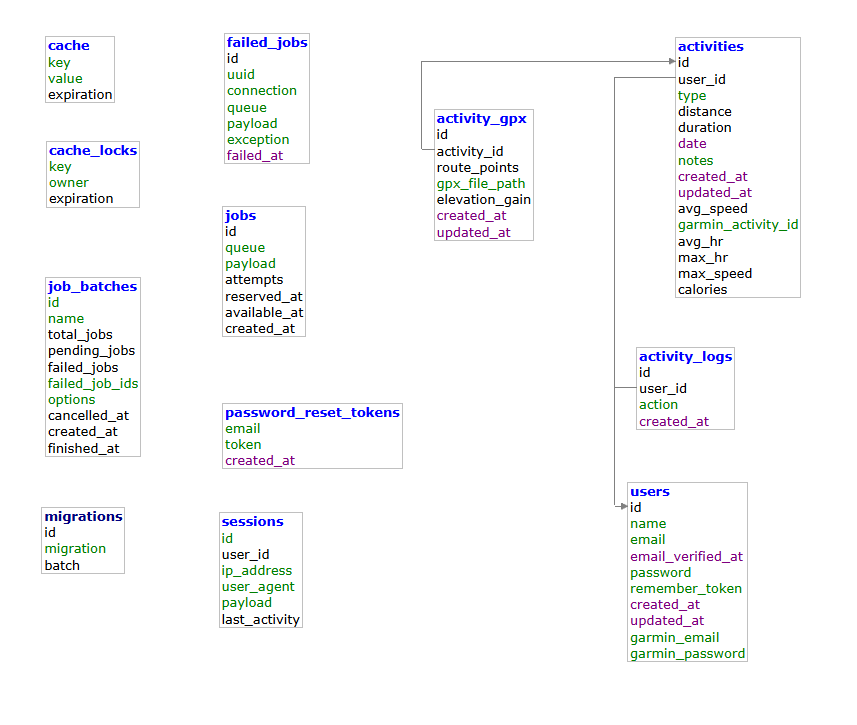
\includegraphics[width=\textwidth]{erd.png}
\caption{Diagram relacji encji bazy danych}
\end{figure}

\section{Więzy integralności}

\subsection{Klucze obce i usuwanie kaskadowe}

Wszystkie relacje między tabelami aplikacyjnymi zabezpieczone są kluczami obcymi z kaskadowym usuwaniem (\texttt{ON DELETE CASCADE}). Oznacza to, że usunięcie rekordu nadrzędnego automatycznie usuwa wszystkie powiązane rekordy podrzędne -- nie ma możliwości pozostawienia osieroconych danych.

\begin{center}
\begin{tabularx}{\textwidth}{|l|l|l|X|}
\hline
\textbf{Tabela} & \textbf{Kolumna FK} & \textbf{Ref. tabela} & \textbf{Zachowanie przy usunięciu} \\
\hline
activities      & user\_id            & users.id             & CASCADE -- usunięcie użytkownika usuwa wszystkie jego aktywności \\
\hline
activity\_gpx   & activity\_id        & activities.id        & CASCADE -- usunięcie aktywności usuwa dane trasy GPS \\
\hline
activity\_logs  & user\_id            & users.id             & CASCADE -- usunięcie użytkownika usuwa jego logi \\
\hline
sessions        & user\_id            & users.id             & SET NULL -- usunięcie użytkownika unieważnia sesje \\
\hline
\end{tabularx}
\end{center}

Dzięki takiej konfiguracji operacja \texttt{DELETE} na tabeli \texttt{users} jest bezpieczna i atomowa -- baza danych gwarantuje spójność bez konieczności ręcznego usuwania powiązanych rekordów w kodzie aplikacji.

\subsection{Ograniczenia unikalności}

\begin{center}
\begin{tabularx}{\textwidth}{|l|l|X|}
\hline
\textbf{Tabela}    & \textbf{Kolumna}      & \textbf{Uzasadnienie}                        \\
\hline
users              & email                 & Każdy adres e-mail może być przypisany do jednego konta \\
\hline
activity\_gpx      & activity\_id          & Jedna aktywność może mieć co najwyżej jeden rekord trasy GPS \\
\hline
failed\_jobs       & uuid                  & Unikalny identyfikator nieudanego zadania kolejki \\
\hline
\end{tabularx}
\end{center}

\subsection{Indeksy}

Poniżej zestawiono indeksy założone na kolumnach najczęściej używanych w klauzulach \texttt{WHERE} i \texttt{ORDER BY}:

\begin{center}
\begin{tabularx}{\textwidth}{|l|l|X|}
\hline
\textbf{Tabela}    & \textbf{Indeksowane kolumny}        & \textbf{Cel}                              \\
\hline
users              & email (UNIQUE)                      & Wyszukiwanie użytkownika podczas logowania \\
\hline
activity\_logs     & action                              & Filtrowanie logów po typie akcji          \\
\hline
activity\_logs     & (user\_id, created\_at)             & Złożony indeks -- pobieranie logów użytkownika posortowanych chronologicznie \\
\hline
sessions           & user\_id                            & Wyszukiwanie sesji należących do użytkownika \\
\hline
sessions           & last\_activity                      & Czyszczenie wygasłych sesji               \\
\hline
cache              & expiration                          & Czyszczenie wygasłych wpisów cache        \\
\hline
jobs               & queue                               & Pobieranie zadań z konkretnej kolejki     \\
\hline
\end{tabularx}
\end{center}

\section{Iteracyjny rozwój schematu bazy danych}

Schemat bazy danych powstawał iteracyjnie -- każda zmiana struktury to osobny, wersjonowany plik migracji. Podejście to gwarantuje pełną historię zmian w repozytorium Git oraz możliwość odtworzenia dowolnego stanu schematu przez uruchomienie migracji w górę (\texttt{migrate}) lub w dół (\texttt{migrate:rollback}).

\begin{center}
\begin{longtable}{|l|p{4.5cm}|p{5.5cm}|}
\hline
\textbf{Data} & \textbf{Plik migracji} & \textbf{Zmiana} \\
\hline
\endhead
2026-03-30 & create\_activities\_table & Pierwsza wersja tabeli \texttt{activities} z kolumnami bazowymi i kolumną \texttt{weather\_json} (JSON) \\
\hline
2026-04-29 & create\_activity\_gpx\_table & Nowa tabela \texttt{activity\_gpx} przechowująca punkty trasy GPS; FK do \texttt{activities} z CASCADE \\
\hline
2026-04-29 & update\_activities\_table & Usunięcie \texttt{weather\_json} (dane pogodowe poza zakresem projektu); dodanie \texttt{avg\_speed} -- normalizacja schematu \\
\hline
2026-05-02 & create\_activity\_logs\_table & Tabela \texttt{activity\_logs} (immutable log zdarzeń) z indeksami na \texttt{action} i \texttt{(user\_id, created\_at)} \\
\hline
2026-05-07 & add\_garmin\_activity\_id & Dodanie \texttt{garmin\_activity\_id} do \texttt{activities} -- klucz obcy do Garmin Connect, zapobiega duplikatom przy synchronizacji \\
\hline
2026-05-07 & add\_stats\_to\_activities & Dodanie kolumn \texttt{avg\_hr}, \texttt{max\_hr}, \texttt{max\_speed}, \texttt{calories} -- rozszerzenie danych ze źródeł Garmin \\
\hline
2026-05-07 & add\_garmin\_credentials\_to\_users & Dodanie \texttt{garmin\_email} i \texttt{garmin\_password} do tabeli \texttt{users} -- przechowywanie zaszyfrowanych danych Garmin \\
\hline
\end{longtable}
\end{center}

Każdy plik migracji implementuje metody \texttt{up()} (aplikacja zmiany) i \texttt{down()} (cofnięcie zmiany), co umożliwia pełny rollback do dowolnego punktu w historii schematu.

\section{Seedery i dane testowe}

\subsection{DatabaseSeeder}

Seeder wypełnia bazę danych wygenerowanymi danymi testowymi, umożliwiając szybkie uruchomienie aplikacji z realistycznym zestawem rekordów bez ręcznego wprowadzania danych.

\textbf{Działanie \texttt{DatabaseSeeder::run()}:}
\begin{enumerate}[noitemsep]
    \item Tworzy (lub odnajduje) stałego użytkownika demonstracyjnego \texttt{nadia@doe.com} z hasłem \texttt{password}.
    \item Generuje 50 aktywności powiązanych z tym użytkownikiem.
    \item Tworzy 100 losowych użytkowników przy użyciu \texttt{UserFactory}.
    \item Generuje 1000 dodatkowych aktywności przypisywanych losowo do wszystkich 101 użytkowników.
\end{enumerate}

Po uruchomieniu seeda baza zawiera łącznie \textbf{101 użytkowników} i \textbf{1050 aktywności}.

\subsection{ActivityFactory}

\texttt{ActivityFactory} generuje realistyczne dane aktywności z użyciem biblioteki Faker:

\begin{center}
\begin{tabular}{|l|l|}
\hline
\textbf{Kolumna} & \textbf{Generowana wartość} \\
\hline
type             & losowo: running / cycling / swimming \\
distance         & losowa liczba zmiennoprzecinkowa 0{,}1--100 km \\
duration         & losowa liczba całkowita 10--300 minut \\
date             & losowa data \\
notes            & losowe zdanie w języku angielskim \\
\hline
\end{tabular}
\end{center}

\subsection{Uruchomienie seederów}

\begin{lstlisting}[language=bash, numbers=none]
# Samo uruchomienie seederów (bez czyszczenia bazy)
php artisan db:seed

# Czyszczenie bazy i ponowna migracja + seed (środowisko deweloperskie)
php artisan migrate:fresh --seed
\end{lstlisting}

% ============================================================

\section{Testowanie i optymalizacja}

\begin{enumerate}[resume]

\item \textbf{Testowanie poprawności operacji CRUD} \\
Każda z czterech operacji na aktywności została zweryfikowana manualnie:
\begin{itemize}[noitemsep]
    \item \textbf{Create} -- ręczne dodanie aktywności przez formularz; weryfikacja zapisu w bazie i wyświetlenia na liście aktywności,
    \item \textbf{Read} -- przeglądanie listy aktywności z filtrowaniem po typie i paginacją; weryfikacja poprawności wyświetlanych danych,
    \item \textbf{Update} -- edycja danych aktywności; weryfikacja zapisu zmian,
    \item \textbf{Delete} -- usunięcie aktywności; weryfikacja kaskadowego usunięcia rekordu z tabeli \texttt{activity\_gpx} oraz pojawienia się wpisu w \texttt{activity\_logs}.
\end{itemize}
Testy przeprowadzono również dla importu z pliku GPX i synchronizacji Garmin, weryfikując poprawność parsowania danych i wykrywania duplikatów na podstawie \texttt{garmin\_activity\_id}.

\item \textbf{Optymalizacja zapytań przez indeksy} \\
Najczęściej wykonywane zapytania zostały zabezpieczone indeksami na poziomie migracji:
\begin{itemize}[noitemsep]
    \item \texttt{users.email} -- indeks unikalny przyspiesza wyszukiwanie użytkownika podczas logowania (operacja \texttt{WHERE email = ?}),
    \item \texttt{activity\_logs(user\_id, created\_at)} -- złożony indeks pokrywający zapytania pobierające logi konkretnego użytkownika posortowane chronologicznie,
    \item \texttt{activity\_logs(action)} -- indeks filtrowania logów po typie akcji.
\end{itemize}
Kolumna \texttt{activities.user\_id} korzysta z indeksu automatycznie tworzonego przez Laravel przy definicji klucza obcego (\texttt{foreignId}), co przyspiesza scopowanie zapytań do zalogowanego użytkownika (\texttt{WHERE user\_id = ?}).

\item \textbf{Normalizacja schematu} \\
W trakcie iteracyjnego rozwoju projektu przeprowadzono normalizację schematu: dane trasy GPS wydzielono do osobnej tabeli \texttt{activity\_gpx} (zamiast przechowywania w kolumnie JSON w tabeli \texttt{activities}). Dzięki temu zapytania do listy aktywności nie pobierają potencjalnie dużych danych trasy -- relacja \texttt{gpxData()} ładowana jest wyłącznie na żądanie (\textit{lazy loading}) przy wyświetleniu szczegółów aktywności. Eliminuje to problem N+1 na liście zbiorczej.

\end{enumerate}

% ============================================================

\end{document}
